\documentclass[12pt,a4paper]{article}
% Packages
\usepackage{graphicx}
\usepackage{amsmath}
\usepackage[hidelinks]{hyperref}
\usepackage{xurl}  % Use xurl for better URL handling
\usepackage{subcaption}  % If using the subfigure approach
\usepackage{setspace}

% pseudocode
\usepackage{algorithm}
\usepackage{algpseudocode}

% tables
\usepackage{tabularx}

\graphicspath{{./images}}
% Title and Author (adjust the spacing as needed)
\title{\LARGE \textbf{CVision}}
\author{Weijing}
\date{\large On: \today}
% Begin Document
\begin{document}
% Title Page
\makeatletter
\begin{titlepage}
\centering
\vspace*{1cm}
 { 
\includegraphics[width=6cm]{logo6.png}}\\[1cm]
 {\LARGE \textbf{CVision: A Navigator for the Visually-Impaired}}\\[0.5cm]
 {\LARGE Winter Quarter Design Packet} \\[1cm]
\textbf{Supervised By:}{ Professor Shivkumar Chandrasekaran}\\[1cm]
\textbf{Written By:}{
 Weijing Wang,
 Jordan Prescott,
 Will Schiff,
 Darren Liu,
 Sayra Salgado,
 Vikram Iyer,
 Rosstin Safavian,
 Angela Cai,
 David Zegarra,
 Mohammed Rehman,
 Theodore Hwang,
 Alperen Yilmaz
 }\\[1cm]
\date{\large Date Last Edited: \today}
 {\@date\\}
\end{titlepage}

% Table of Contents
\tableofcontents
\clearpage

\section{Executive summary}
CVision is a Python computer program that aims to assist the visually-impaired with navigating surroundings.
The users of this program will listen to spatial audio from headphones that is generated based on the video feed from a portable camera such as a modern phone.
Through the spatial sound, the user will be able to determine the identity and relative locations of objects, track specific objects, and be warned about anything which poses potential dangers to the user. 
Fig. \ref{our_vision} below shows how we envision our final product to look like.
In this Figure, the user is shown to use a phone to run CVision.
However due to the current technology limitations and our budget, we are planning to use a GPU laptop for our final demonstration.

\begin{figure}[ht!]
    \center
    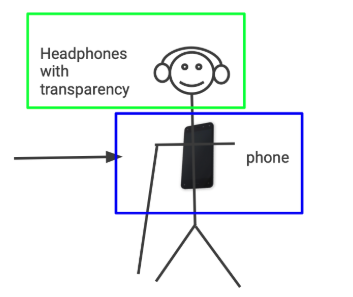
\includegraphics[width=0.7\linewidth]{our_vision.png}
    \caption{CVision would ideally run on a device like a phone which the user can point around to hear their surroundings.}
    \label{our_vision}
  \end{figure}

% Our report will first go over:
% Title page, Table of contents, Executive summary
% Introduction: why we need our thing
% Competitions existing products → what we need in our design
% What we features we want our design to have
% What we decided on: Working of our design
% General overview
% Block diagram of design
% Brief explain each block
% Parts of our design details
% Depth and why we chose DepyhAnythingv2metric over MoGe, depth pro for now
% Object detect and why we chose YOLOv8 over SAM grounded sam, etc
% Sound generation
% Justification
% GloVE explanation and what it might be used for and pros and cons
% Budget
% Current demo state
% Next steps
% Say we need to do more testing and make the demo work for more things
% Should be able to handle multiple objects and the outdoors, and manage low frame rate
% Timeline. Gantt chart

\newpage
\section{Introduction/Background}
Visually impaired individuals have long relied on tactile and auditory aids like canes and guide dogs, which provide essential but limited information about dynamic environments.
Advances in AI and machine learning now offer new opportunities to enhance spatial awareness through real-time depth perception, object detection, and auditory scene description.
Recent models such as DepthAnythingV2 and DepthPro enable depth estimation, while YOLOv8segn and ByteTracker with IoU provide real-time object detection and tracking. These technologies create the foundation for AI-driven assistive tools that describe surroundings through spoken feedback, improving navigation and environmental understanding.
We would like to create a program that take advantage of these recent advancements to improve the experience for the visually-impaired.

\subsection{Existing Solutions and Limitations}

Several products are already taking advantage of the recent AI computer vision advancements, including:

\begin{figure}[ht!]
    \centering
    \begin{minipage}[t]{0.65\textwidth}
        \centering
        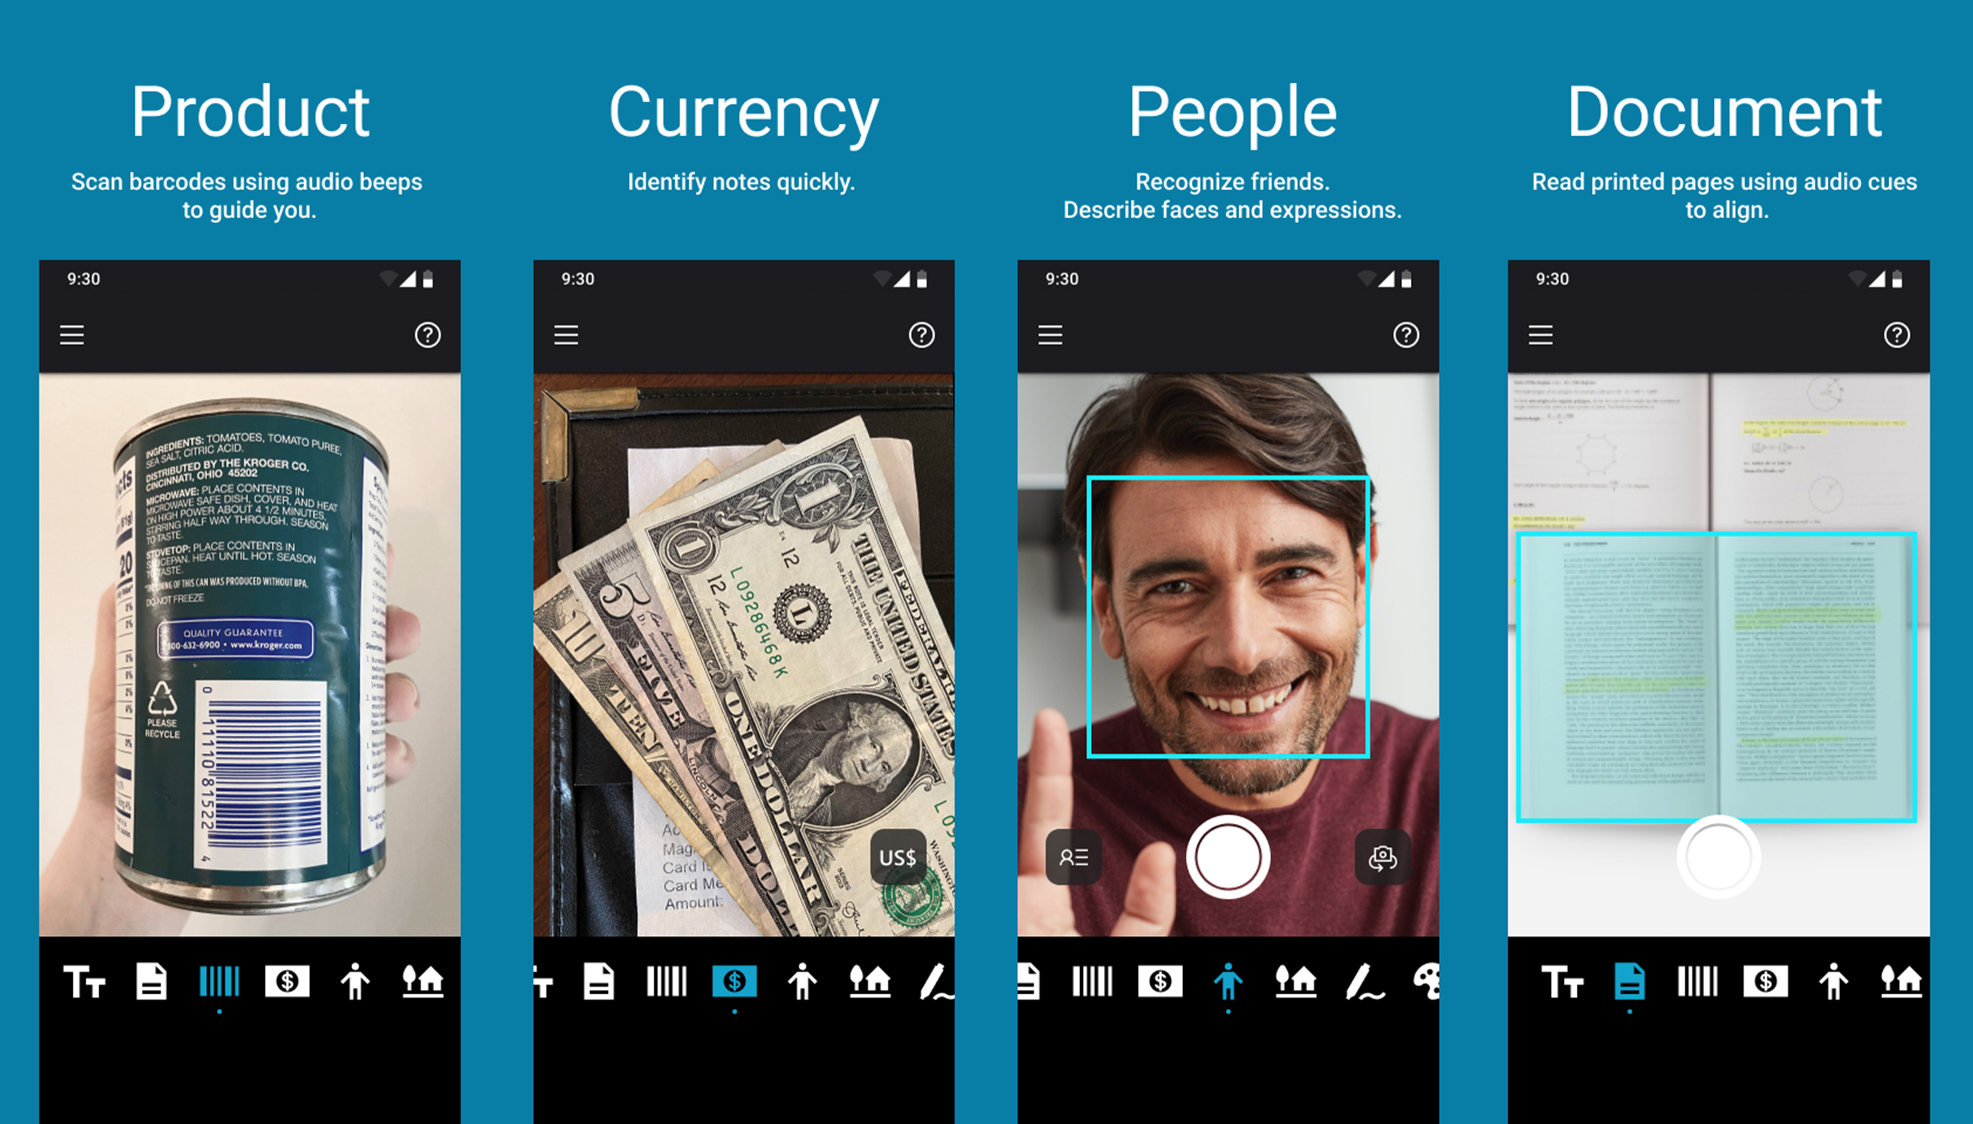
\includegraphics[width=\textwidth]{Seeing-AI-Android-channels.png}
        \caption{Microsoft Seeing AI can read product descriptions, currency documents and recognize faces \cite{microsoft2025}}
        \label{seeingai_pic}
    \end{minipage}%
    \hfill
    \begin{minipage}[t]{0.3\textwidth}
        \centering
        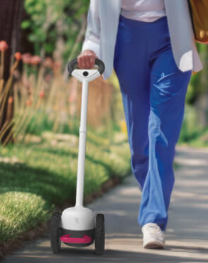
\includegraphics[width=\textwidth]{glidance.png}
        \caption{Glidance's Glide guides users on roads and to destinations \cite{glidance}}
        \label{glidance_pic}
    \end{minipage}
\end{figure}

\begin{enumerate}
    \item Microsoft Seeing AI: known as the "Swiss army knife for blind people" \cite{microsoft2024}, Seeing AI can perform tasks such as scene description, text reading, or reading currency as shown in Fig. \ref{seeingai_pic}
    It also has many experimental features such as real-time object detection and navigation. As these features are experimental, they are not very useful because of the limited amount of things it can detect and inaccuracies.
    \item Be My Eyes: A platform where visually-impaired users can call volunteers to help with daily tasks \cite{bemyeyes}. This is useful, but may be hard to use due to the human contacts.
    \item Envision AI: Similar to Seeing AI, but also offers smart glasses for object, text, and facial recognition. It can run offline, but it is less accurate than when it is connected to the internet \cite{envision}.
    \item Glidance's Glide: A walking stick with wheels on the bottom that can guide users on roads and detect entrances/exits and obstacles as shown in Fig. \ref{glidance_pic}. From their preorder website, it seems well-designed, but may suffer from rough terrain. It is also not as accessible because it is around \$30 USD per month \cite{glidance}. 
\end{enumerate}
While effective, these solutions are limited in their usability in complex scenarios like obstacle navigation and street crossing.
Furthermore, many of them suffer from inaccuracies and small set of objects able to be detected due to the limitations of the computer vision technology they might have used.
Finally, besides Glidance, none of the existing solutions have a function which can automatically warn the user of potential dangers.

\newpage
\section{Design of product}
Our system differentiates itself by running locally without internet dependence.
It also takes on the challenge of real-time navigation and object tracking by leveraging the latest AI computer vision advancements, something that has remained in its experimental or starting stages in our competitors.
CVision will acquire accurate information from our camera input using state-of-the-art neural networks which will generate the spatial audio descriptions.
By doing this, we will enhance environmental perception, allowing visually impaired users to navigate complex settings with greater confidence and safety than ever before.
\subsection{Product Definition}
The final product will be a system which translates the surrounding environment and obstacles/objects in the vicinity into audio cues to give the user real-time spatial awareness through their headphones.
To do this, the input data from the portable camera is processed as shown in Fig \ref{data_flow} to get object distance and relative location to the user and object name.
This is done with depth estimation and object recognition neural networks to produce the necessary information from the surrounding environment.
This information is finally passed through signal processing techniques to describe the scene accurately and provide cues to the user to navigate the scene. 

\begin{figure}[ht!]
    \center
    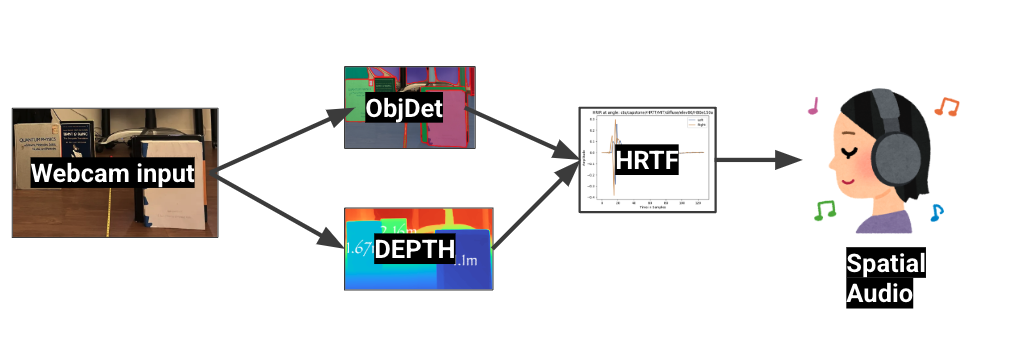
\includegraphics[width=1\linewidth]{data_flow.png}
    \caption{CVision input data flow.}
    \label{data_flow}
  \end{figure}
\newpage
To run all this code, we will use a GPU computer, even though the end goal is to be on a portable device, so that it can maintain a high enough FPS (~10 FPS) to be useful and to prove the concept.
Additionally, we envision using voice activation for user input, but for now, we will use text commands for demonstration purposes as shown in Fig. \ref{gui}.
Our table of needs, target specifications and Engineering Characteristics is shown in Table \ref{tab:needs_specs}.

\begin{figure}[ht!]
    \center
    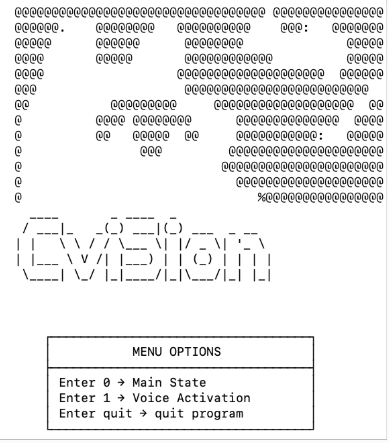
\includegraphics[width=0.43\linewidth]{gui.png}
    \caption{CVision current terminal based interface.}
    \label{gui}
  \end{figure}


  \begin{table}[htbp]
    \centering
    \caption{Needs, Target Specifications, and Engineering Characteristics}
    \label{tab:needs_specs}
    \begin{tabularx}{\textwidth}{|l|X|X|}
    \hline
    \textbf{Needs} & \textbf{Target Specifications} & \textbf{Engineering Characteristics} \\
    \hline
    Depth Map & Accurately determine depth of environment surroundings in meters & Monocular depth neural network and traditional computer vision techniques \\
    \hline
    Object Recognition & Identify objects in image & Object classification and segmentation neural network \\
    \hline
    Audio Output & Stereo spatial audio & Audio processing, Head related transfer function (HRTF) \\
    \hline
    \end{tabularx}
    \end{table}

\newpage
\subsection{Concepts and Systems}
To ensure our program works, we designed our state chart shown in Fig. \ref{states} to be as simple as possible.
It has 3 modes: NORMAL, TRACKING and DANGER.
The default mode is NORMAL where new detected objects will be announced in their corresponding spatial locations.
If the user selects one of the detected objects, TRACKING is activated and will play a tone in the correct spatial location until the user is guided to the object.
Finally, if at any point the program detects any danger in the dangerous objects list or and objects too close, DANGER is automatically activated and will stop everything to warn the user about the danger by playing a warning tone at the corresponding locations.
Once the danger is gone, the program returns to the NORMAL state.
Our implementation of this state chart for each frame in the input video is shown as pseudocode in Alg. \ref{alg:grandloop}.
\begin{figure}[ht!]
    \center
    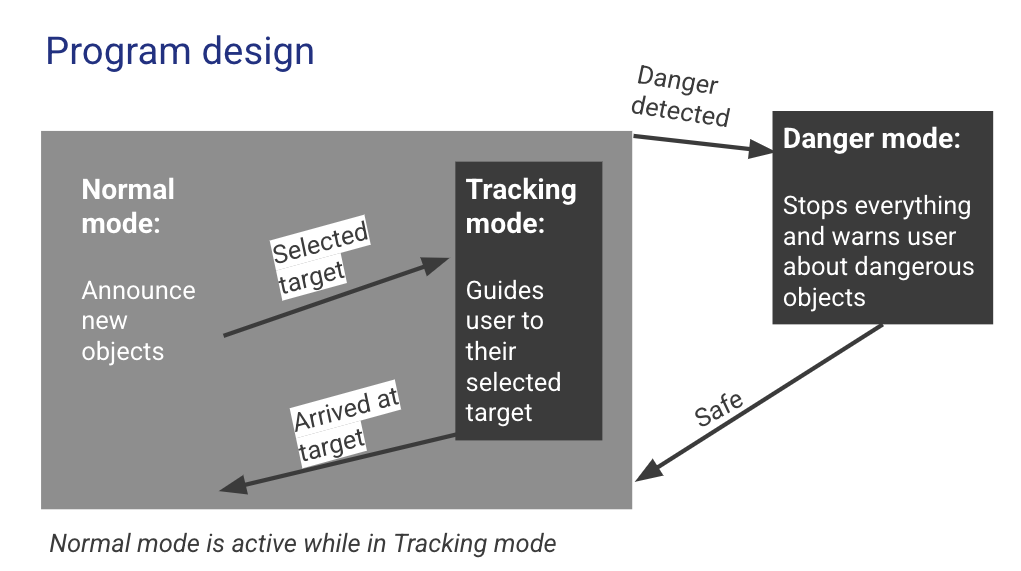
\includegraphics[width=1\linewidth]{state_diagram.png}
    \caption{CVision program state chart with states NORMAL, TRACKING, and DANGER}
    \label{states}
  \end{figure}
  \newpage

  \begin{algorithm}
    \caption{CVision Main loop}
    \label{alg:grandloop}  % Label for referencing
    \begin{algorithmic}[1]
        \While{True}
            \State Get frame, depth map, and detect objects/segment
            \If{any objects are too close or dangerous}
                \State Enter DANGER
            \EndIf
            \If{DANGER}
                \State Continuously play all the dangerous objects' names spatially
            \Else
                \State Announce any new objects that appear spatially (NORMAL)
            \EndIf
            \If{inputted target to track}
                \State Play sine sound at target location until distance to target is 1 meter (TRACKING)
            \EndIf
        \EndWhile
        \end{algorithmic}
        \end{algorithm}



        
        \subsection{Must-Have Features}
        The product is intended to provide audio cues in real-time, meaning that the scene should be captured, processed, and converted to audio quickly enough for the user to react to the changing environment.
        Therefore, the minimum performance specs that need to be met by final product should be around 10 FPS.
        A table of minimum specifications for our system is shown in Table \ref{tab:min}. Our Design Component Requirements are in Table \ref{tab:comp_describe}.

        Monocular depth estimation and object recognition are necessary specifications of the product, to a high level of accuracy. Additionally, sound processing and descriptive audio cues are fundamental necessities of the product. This includes differentiating between objects in terms of urgency to the user. For example, when alerting the user of objects that could cause harm to the user, a car moving towards the user would take priority over a stationary object several meters away. 
        In order to achieve high efficiency of the system, the text-to-speech/audio output subsystem will leverage the results of both the object recognition and depth map outputs, which will run in parallel. The results needed for the sound output subsystem to produce an accurate description of the environment include the object classifications, depths of each object from the camera, and the angle relative to a point directly in front of the user. This will allow for not only accurate identification of objects, but a stereo-panned output cue indicating where exactly the object is. 

        \subsection{Preferred Features and Stretch Goals}
        The primary preferred feature is to push the speed of the system to allow for more accurate scans of the world around the user. Should the system be able to be optimized to a one or two second runtime, then the pictures that will be processed into surrounding information will be at that frequency. While it is very unlikely that the system will be fast enough to run multiple images a second, having a runtime of about a second will give a much better picture of the surrounding environment than a runtime of 10 seconds, which would be useful but much more limited. Additionally, we are hoping to use computer vision based techniques to confirm ground truths, and use these measurements that don’t have the inherent uncertainty of neural networks to ensure that our neural network outputs are accurate to a reasonable degree. A final preferred feature is to create an interface for users who are not fully blind, and use this interface to display much more information than would be possible to reasonably convey with our audio output.


        \begin{table}[h!]
            \centering
            \caption{Design Performance Minimum Requirements}
            \begin{tabular}{|l|p{10cm}|}
            \hline
            \label{tab:min}
            \textbf{Component} & \textbf{Minimum Specification} \\ \hline
            Image Resolution & 1080p (subject to adjustment based on further testing). \\ \hline
            Processing Power & NVIDIA RTX 1000 Ada, Intel Core Ultra 7 155H, 32GB LPDDR5X, 512 GB SSD \\ \hline
            Depth Accuracy & ±0.5m for effective spatial awareness. \\ \hline
            Audio Output & TTS should support volume and stereo positioning for directional feedback. \\ \hline
            Power & Portable battery supporting 4+ hours of operation. \\ \hline
            \end{tabular}
            
            \end{table}

            \begin{table}[h!]
                \centering
                    \caption{Design Component Requirements}
                \label{tab:comp_describe}
                \begin{tabular}{|l|p{10cm}|}
                \hline
                \textbf{Component} & \textbf{Description} \\ \hline
                Camera Module & Captures high-resolution images (1080p) for reliable object recognition and depth estimation. \\ \hline
                Processing Unit & Performs real-time image processing and depth estimation. The NVIDIA Jetson Nano or Jetson Xavier is recommended for real-time performance. \\ \hline
                Depth Sensor & Provides pixel-level depth data. Apple Depth Pro or similar pre-trained network is used. \\ \hline
                Recognition Module & Object detection via YOLO for fast, reliable identification and classification of objects. \\ \hline
                Audio Processing Unit & Converts JSON data into spatial audio cues using text-to-speech with volume and stereo adjustments. \\ \hline
                Power Source & Portable battery compatible with processing unit for extended, mobile operation. \\ \hline
                Speaker/Headphone Output & Outputs audio cues to user with volume and directional cues for spatial awareness. \\ \hline
                \end{tabular}
                \end{table}

\newpage
\section{Important Concepts}
The following are the key concepts present in CVisions input data flow as referenced in Fig. \ref{data_flow} and will be expanded on in this section:
\begin{enumerate}
    \item Object detection: Identifies objects in the scene and their horizontal and vertical placements in the frame.
    \item Depth Estimation: Measures the distance of objects, enabling spatial awareness.
    \item Sound module: generates spatial sound based on output data from depth and object detection modules.
    \item User experience: some experimental features we are working on to address potential safety concerns and to improve user experience.
\end{enumerate}



\subsection{Object Detection Module}
This module will take in the input frame and return all the objects in the frame with their locations and class names.
We use the pre-trained YOLO neural network for object recognition. YOLO acts as a "black box," taking an input image and returning detected objects within it. It also returns a bounding box around each detected object as shown in Fig. \ref{yolo} \cite{redmon2018yolov3}. This approach simplifies the process, as the network can identify objects without requiring additional training.

\begin{figure}[ht!]
    \center
    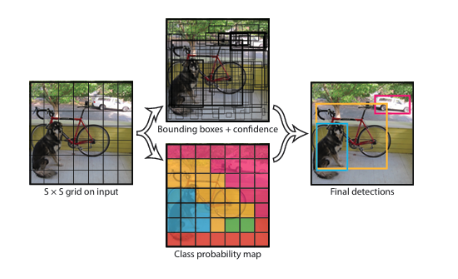
\includegraphics[width=1\linewidth]{yolo.png}
    \caption{YOLO boxes all the objects it detects.}
    \label{yolo}
  \end{figure}

We ultimately chose YOLOv8-seg over other segmentation models because it has balance between accuracy, speed, and ease of implementation \cite{ultralytics2024sam}. While other segmentation models like FAST-SAM tend to not be so ideal for real-time processing, YOLOv8-seg, on the other hand, provides instance segmentation in order to not only capture an object but its boundaries in challenging settings. Additionally, its active development and vast documentation provides us ease in troubleshooting, optimizing performance, and finding compatible datasets for which we might want to train \cite{ultralytics2024sam}. This ensures that our model effectively recognizes objects like sidewalks, cars, roads, and bikes as it will ultimately improve navigation assistance for visually impaired individuals.

\subsection{Depth Map Module}
A depth map shows the distance of each pixel in a picture to the camera taking the picture. We get a depth map from Monocular metric estimation depth maps using deep neural networks.

In choosing our depth map network, we came to a decision between 2 networks- Depth Anything v2 and Depth Pro. Depth Pro has the huge advantage of being the most accurate and consistently accurate, but with a large tradeoff of having a much larger runtime \cite{bochkovskii2024depth}, as it is a much larger model then Depth Anything v2. Depth Pro also has the advantage of converting its relative depth calculations into absolute depth (in meters rather than relative other locations in input images) which allows us to get more accurate and helpful results. However, Depth Pro is much slower than Depth Anything v2, so we leave open the opportunity to implement Depth Anything as a “fast mode” should the much quicker runtime be desired, however, Depth Pro’s accuracy is so superior and boasts so much higher stability compared to other models that in general use cases we default to Depth Pro.

\subsection{Combining Object Detection and Depth Information}
After acquiring object and depth data, we analyze specific depth ranges to identify objects at those distances. This approach ensures that closer features, such as protruding parts of an object, are detected and accurately mapped to the user. For example, if a tank is facing the user with its barrel pointed forward, taking the average depth could ignore the barrel’s proximity. By analyzing depth ranges, we ensure that the system detects the closer barrel rather than the tank's main body.

\subsection{Relative Angle Calculation}
The relative angle of each detected object is determined using the bounding box coordinates provided by YOLO. The horizontal value of the bounding box's center is taken and then normalized by the image width, resulting in a value from 0 (far left) to 1 (far right).

\newpage
\subsection{Sound Module}
The sound module takes in the depth, location class name data of each object, finds the sound file of that object name and plays it through the HRTF.
Then we get the spatial audio. In other words, after getting the label, depth, and angle values, they are converted into JSON format and passed to the text-to-speech (TTS) module. This module processes the depth and angle data to create a stereo sound that describes each object and its distance from the user. The TTS output adjusts volume based on object distance (quieter for farther objects) and pans audio to the left or right based on the object's relative angle, giving the user a spatial audio experience.
\subsubsection{Head Related Transfer Function (HRTF)}
In order to accurately convey three-dimensional object data, we output spatial audio to the user with head-related transfer functions.
Research institutions such as MIT generate datasets of impulse responses like in Fig \ref{HRTF} by measuring the response of a speaker placed at different positions around the room as shown in Fig \ref{HRTF_diag}.
These responses depend on the distance from the microphone to the speaker, as well as the azimuth angle.
We convolve the text output with the impulse response that most closely aligns to the object’s position, giving an accurate audio representation of the environment.
\begin{figure}[ht!]
    \centering
    \begin{minipage}[t]{0.55\textwidth}
        \centering
        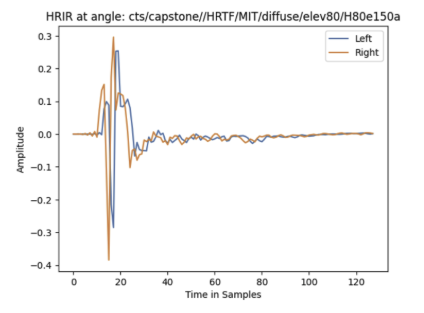
\includegraphics[width=\textwidth]{HRTF_func.png}
        \caption{One of the HRTFs from MIT}
        \label{HRTF}
    \end{minipage}%
    \hfill
    \begin{minipage}[t]{0.4\textwidth}
        \centering
        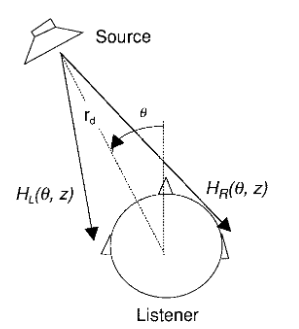
\includegraphics[width=\textwidth]{HRTF_man.png}
        \caption{How HRTF is made}
        \label{HRTF_diag}
    \end{minipage}
\end{figure}

\newpage
\subsection{User Experience}
\subsubsection{Ranking dangerous objects in order of danger using GloVE}
To systematically determine the urgency level of detected objects and subsequently prioritize audio output, our project integrates GloVe (Global Vectors for Word Representation) embeddings, a widely-used semantic representation model developed by Stanford NLP \cite{pennington_glove}. GloVe embeddings map words into high-dimensional vector spaces, encoding semantic relationships based on the co-occurrence of words within large textual corpora. By leveraging these semantic embeddings, our system identifies and prioritizes detected objects according to their semantic similarity to predefined categories known to pose varying levels of immediate risk to visually impaired users. By comparing detected objects to predefined categories such as vehicles, the system dynamically classifies objects as urgent or non-urgent. Urgent objects, particularly vehicles, trigger prioritized audio alerts—adjusting in frequency, waveform, and volume—to clearly inform users of immediate dangers.

\begin{figure}[ht!]
    \center
    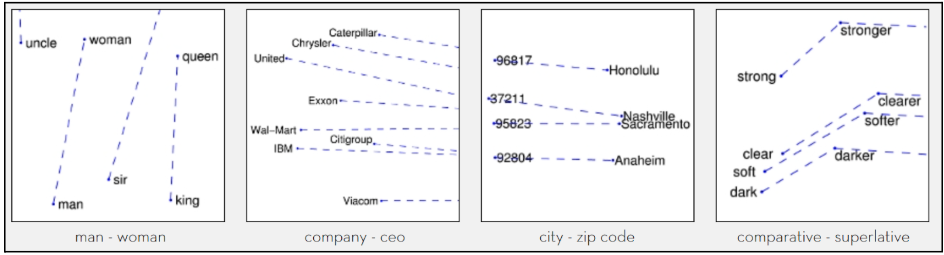
\includegraphics[width=1\linewidth]{glove.png}
    \caption{GloVe Word to Vector Implementation}
    \label{glove}
  \end{figure}
\subsubsection{User feedback}
Efforts were made to come into contact with the local Braille Institute in downtown Santa Barbara, however, they did not respond to any outreach. The Test and Evaluation team then decided to reach out to the Los Angeles Braille Institute branch, and send them a survey to receive customer feedback. This process is still ongoing and will continue through Spring Quarter. 





\newpage
\section{Risk Analysis}
This section details our risk analysis. Our risk analysis chart is shown in Table \ref{tab:risk-assessment}.

\begin{table}[htbp]
    \centering
    \caption{Risk Analysis Chart}
    \label{tab:risk-assessment}
    \begin{tabular}{|p{3cm}|c|c|p{6cm}|}
    \hline
    \textbf{Risk Factor} & \textbf{Likelihood} & \textbf{Impact} & \textbf{Mitigation Strategy} \\
    \hline
    Technology Limitations & High & High & Improve models by iterating through different algorithms and prototypes \\
    \hline
    User Experience & Medium & High & Conduct series of testing with blind users and gather feedback \\
    \hline
    Portability & Medium & Medium & Find energy efficient algorithms and models \\
    \hline
    Reliability & Medium & High & Thorough testing using multiple edge cases and various testing sets \\
    \hline
    Accessibility & High & High & Simplify models and algorithms to be able to run on simple devices \\
    \hline
    \end{tabular}
    \end{table}

\textbf{Technology Limitations:}
Converting visual information via synchronization of information from object recognition, image processing, and depth sensing at high speeds with current technology is difficult. Converting complex scenes into understandable audio cues at real-time is extremely challenging. 

For instance, recognizing high-speed moving objects and their direction is critical for users. LIDAR and stereo cameras are expensive and energy-intensive. Our products should also be an in-hand device, so attaching extra pieces to that is an issue.

\textbf{User Experience and Usability:}
Designing a UI that is friendly for blind users without overwhelming them is complex. Blind users need a friendly interface to navigate and interpret the information outputted to them at a continuous rate. 

Overloading the user with too much auditory feedback could lead to fatigue and confusion, causing more harm, especially in crowded and complex scenes such as busy streets or crowded roads. Finding the right balance is crucial to providing a safe, secure, comfortable, and effective experience.

\textbf{Energy Efficiency:}
The device is meant to be portable, so it has to be energy-efficient while providing high performance. Processing data in real-time uses a lot of energy, which may require extra hardware for additional battery life. This additional hardware could reduce portability, so the design of our program should be energy-efficient.

\textbf{Reliability:}
The product is intended to help the user. Therefore, the safety of the user is the highest priority. Misinterpreting any data could lead to unsafe and dangerous situations, such as missing a high-speed car.

\textbf{Accessibility:}
The technology and processing power required for the program require expensive equipment. This creates an issue for affordability and widespread use. High costs will likely make the product inaccessible, especially to those who would benefit from it the most. 

Adding additional hardware for the sake of accuracy and faster processing will drive up device costs. Finding affordable techniques could reduce costs but may be more of a developmental burden.

\textbf{Unknowns to Address/Verify:}
Sensory Feedback: Look to understand the best sort of audio feedback for the user. This must have enough information to convey complex scenic information, but also simple enough to not overwhelm the user. 

\textbf{Environmental Variance:}
The device should be able to function properly under different environments and conditions. Some examples are low-light, extremely bright light, rain, high-traffic areas, etc. 

\newpage
\section{Current Prototype}
Here is the progress of our current prototype. The NORMAL, TRACKING and DANGER modes from the state chart in Fig. \ref{states} are all implemented in real-time on a GPU computer in Python.
The screenshots here are all running on a Mac, so it is running at ~3FPS, but it runs closer to 12FPS on our GPU laptop.
In NORMAL mode as shown in Fig. \ref{normal_mode}, all the objects are shown to be boxed and segmented in the top right. The depth map is also shown there. On the bottom, all the object data is shown for debug purposes.
The TRACKING mode in Fig. \ref{tracking_mode} is also implemented, and the current target object is the person with class ID 1. The person is also segmented on the right. A tone is being played with volume proportionate to the distance of the person to the camera.
Finally, the DANGER mode in Fig. \ref{danger_mode}, and instead of a green color for the segmentation, it is now red to indicate that the person is closer than 1 meter from the camera. It will also turn red for any objects that we define as dangerous in a predefined list of dangerous class names.

\begin{figure}[ht!]
    \center
    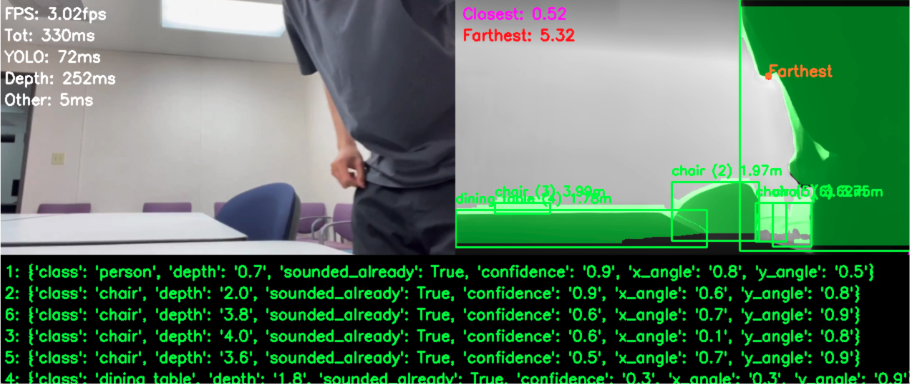
\includegraphics[width=1\linewidth]{normal_mode.png}
    \caption{CVision NORMAL mode. All newly detected objects are announced through spatial audio.}
    \label{normal_mode}
  \end{figure}

\newpage
\begin{figure}[ht!]
    \center
    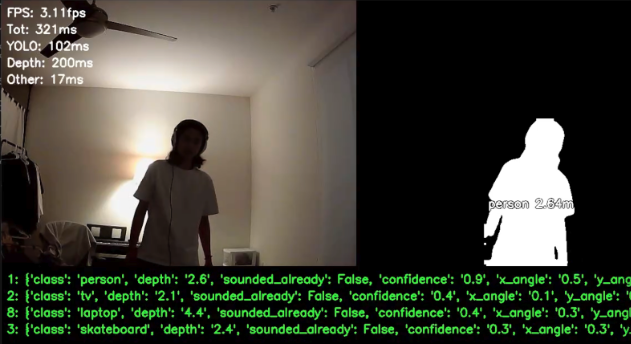
\includegraphics[width=1\linewidth]{tracking_mode.png}
    \caption{CVision TRACKING mode. The tracked object is shown as the mask and the tone is played at its location.}
    \label{tracking_mode}
  \end{figure}


  \begin{figure}[ht!]
    \center
    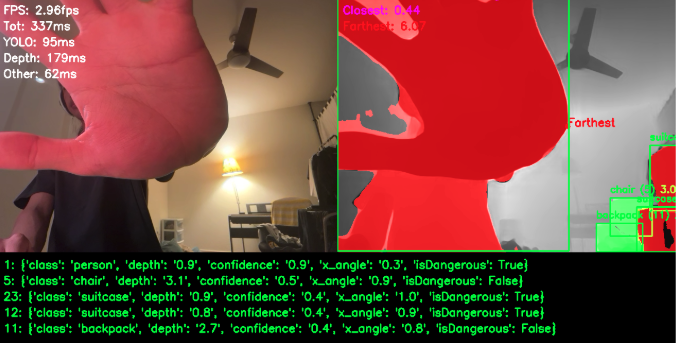
\includegraphics[width=1\linewidth]{danger_mode.png}
    \caption{CVision DANGER mode. Dangerous objects are colored red and a warning tone is played for all the objects at their locations.}
    \label{danger_mode}
  \end{figure}


\newpage
\section{Task Distribution}
Since our project covers a lot of different topics, we decided to split into 4 subteams as shown in Fig. \ref{team}. Those being: Object Recognition, Depth Map, Sound Output, Test/Evaluation. We did not see the need for individual leaders in each group, as we all communicate effectively and function well enough together. Hence, there was no need for an additional hierarchical system to be placed. Each team reports weekly updates to our professor, who is the sponsor for our group, and also answers any related questions we have on the project.
\begin{figure}[ht!]
    \center
    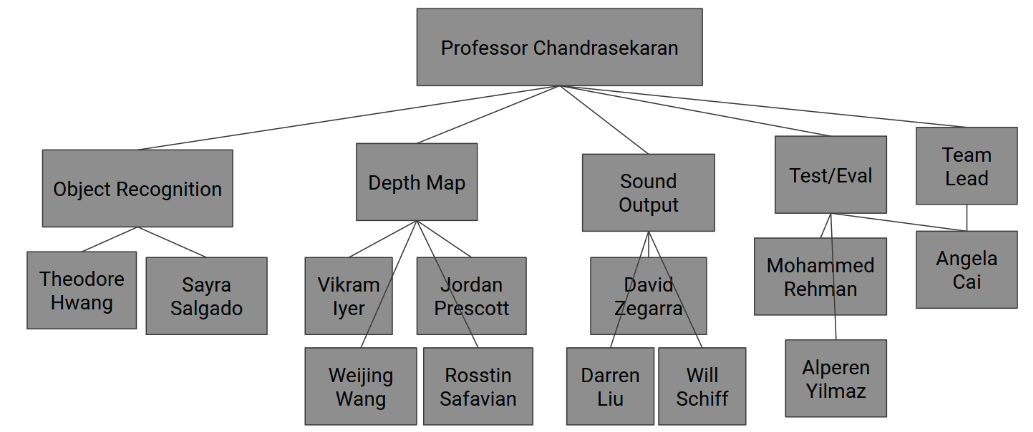
\includegraphics[width=1\linewidth]{team.png}
    \caption{CVision team structure}
    \label{team}
  \end{figure}

\subsection{Object detection team}
The goal of the object recognition team is to determine the number of objects in any scene, identify and classify each and every object. To do this, they implement models with artificial intelligence(e.g. YOLOv8) and research more on topics such as neural networks, image segmentation, and object classification. They also must integrate their work with the depth map team, saving their results as a json file that can be used by the sound team. 

\subsection{Depth Team}
The goals of the depth map team are to accurately determine the depth of the surroundings, and produce an array of distances for each pixel in the image. They do this by researching and using Apple depth pro and perform angle calculations. Furthermore, they integrate their work with the object recognition team to produce refined spatial audio results for the sound team. 

\subsection{Sound output team}
The goals of this team are to give accurate verbal cues for objects at each location, prioritizing those that present more of a danger to the user's life. They do this by using the outputs of the object recognition team and the depth map team to create spatial audio output for the verbal cues. They also research and implement Piper TTS and other HRTF models \cite{rhasspy2024piper}.

\subsection{Test/Evaluation team}
The goals of this team are to provide the other subteams with images or locations that can be evaluated effectively. They create their own metric system to judge the other teams on their performance, and challenge the other teams to overcome obstacles in their work. Additionally, test and evaluation reach out to third parties for product testing and customer feedback to improve testing and the product itself.

\section{Budget}
This project consists mainly of software tools that are available to all members of the group. The amount of computation occurring within the project requires hardware processing power available within the GPU Lab and from our team members' laptops. This quarter we found the software needed stronger hardware for testing and for the team to have a laptop that we could use whenever we needed to. 
So far, we have bought a GPU laptop and a webcam for demo purposes. We don't expect to spend anymore. Our current expenses total up to \$2357.49 USD and are shown in Table \ref{tab:expenses}.

\begin{table}[htbp]
    \centering
    \caption{Total Expenses}
    \label{tab:expenses}
    \begin{tabular}{|l|c|r|r|}
    \hline
    \textbf{Item} & \textbf{Quantity} & \textbf{Unit Price} & \textbf{Total} \\
    \hline
    dell mobile precision workstation 5690  & 1 & \$2,327.49 & \$2,327.49 \\
    \hline
    Logitech Brio 100 Webcam & 1 & \$30.00 & \$30.00 \\
    \hline
    \hline
    \multicolumn{3}{|r|}{\textbf{Grand Total}} & \$2357.49    \\
    \hline
    \end{tabular}
    \end{table}

\newpage
\section{Next steps}
Now we have a working demo, however it still has some issues such as having problems with multiple objects with the same class, overcrowded rooms, and occasional audio glitches.
We don't think they will take too much time and can be properly addressed in the first three weeks of Spring quarter. Additionally, we will also do extensive testing on some specific cases such as choosing the correct objects out of three objects on a table.
The Spring quarter schedule is shown in Fig. \ref{gant}. The full Gantt chart for the entire year is shown in Fig. \ref{full_gant}.
\begin{figure}[ht!]
    \center
    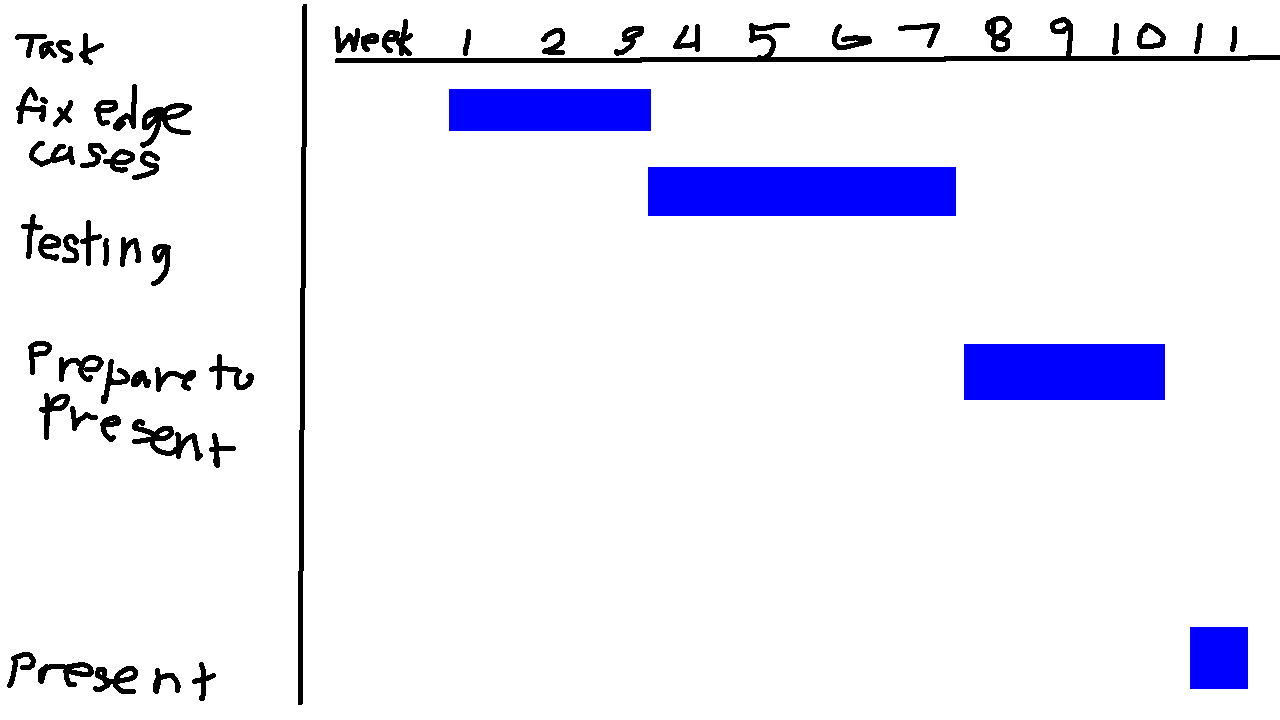
\includegraphics[width=1\linewidth]{gant.png}
    \caption{CVision Spring Quarter schedule}
    \label{gant}
  \end{figure}

\begin{figure}[p]
    \vspace*{-2cm}  % Adjust this value to move the image higher on the page
    \centering      % Note: \center is deprecated, use \centering instead
    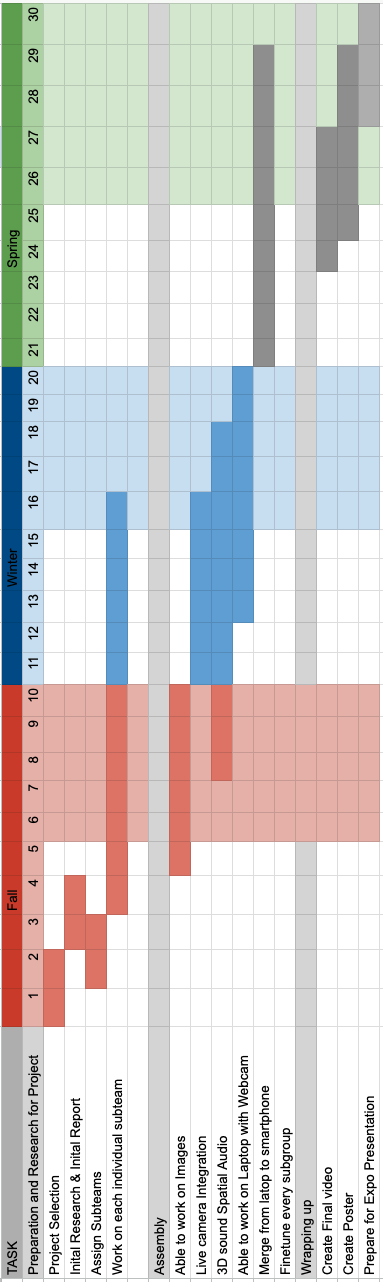
\includegraphics[width=0.49\linewidth]{full_gant.png}  % Use full linewidth instead of 0.42
    \caption{CVision full year Gantt chart}
    \label{full_gant}
    \vspace*{\fill} % This pushes everything above it to the top of the page
\end{figure}

\newpage
\begin{thebibliography}{9}
    
    \bibitem{microsoft2024} 
    Microsoft AI Blog. 
    "Decades of Computer Vision Research: One Swiss Army Knife."  
    Available at:  
    \url{https://blogs.microsoft.com/ai/decades-of-computer-vision-research-one-swiss-army-knife/}.
    
    \bibitem{microsoft2025} 
    Microsoft Accessibility.  
    \textit{Seeing AI App Launches on Android, Including New and Updated Features and New Languages}.  
    Available at: \url{https://blogs.microsoft.com/accessibility/seeing-ai-app-launches-on-android-including-new-and-updated-features-and-new-languages/}.  
    Accessed: March 7, 2025.

    \bibitem{bemyeyes} 
    Be My Eyes.  
    \textit{See the World Together}.  
    Available at: \url{https://www.bemyeyes.com}. Accessed: March 7, 2025.

    \bibitem{envision} 
    Let's Envision Support.  
    \textit{Which features work without an Internet connection?}  
    Available at: \url{https://support.letsenvision.com/hc/en-us/articles/4437254114449-Which-features-work-without-an-Internet-connection}.  
    Accessed: March 7, 2025.

    \bibitem{glidance} 
    Glidance.  
    \textit{Hands-free mobility for the blind and visually impaired}.  
    Available at: \url{https://glidance.io}.  
    Accessed: March 7, 2025.

    \bibitem{pennington_glove} Pennington, J., Socher, R., \& Manning, C. D. (n.d.). GloVe: Global vectors for word representation. Stanford NLP Group. Retrieved March 7, 2025, from \url{https://nlp.stanford.edu/projects/glove/}.

    \bibitem{bochkovskii2024depth} Bochkovskii, A., Delaunoy, A., Germain, H., Santos, M., Zhou, Y., Richter, S. R., \& Koltun, V. (2024). Depth Pro: Sharp Monocular Metric Depth in Less Than a Second. \textit{arXiv e-prints}, arXiv:2410.02073. \url{https://doi.org/10.48550/arXiv.2410.02073}.

    \bibitem{redmon2018yolov3} Redmon, J., \& Farhadi, A. (2018). YOLOv3: An Incremental Improvement. \textit{arXiv}. Retrieved from \url{https://arxiv.org/abs/1804.02767}.

    \bibitem{rhasspy2024piper} Rhasspy Project. (2024). Piper: A fast, local neural text-to-speech system. \textit{GitHub}. Retrieved October 25, 2024, from \url{https://github.com/rhasspy/piper}.

    \bibitem{ultralytics2024sam} Ultralytics. (2024, October 14). SAM (Segment Anything Model). \textit{Ultralytics YOLO Docs}. Retrieved from \url{https://docs.ultralytics.com/models/sam/}.

    \end{thebibliography}
    


\end{document}